\documentclass{beamer}

\usepackage{amsmath}
\usepackage{graphicx}
\usepackage{hyperref}

\title{String Theory and M-Theory: the Theory of Everything}
\author{Donald Leung}
\institute{Kellett School}
\date{\today}

\begin{document}

\begin{frame}
\titlepage
\end{frame}

\begin{frame}
\frametitle{Table of Contents}
\tableofcontents
\end{frame}

\section{Special and General Relativity}

\begin{frame}
\frametitle{Special and General Relativity}
\end{frame}

\begin{frame}
\frametitle{Background History}

\begin{itemize}
\item Published by Albert Einstein
\item Published in 1915
\item Theory of Gravitation
\end{itemize}

\end{frame}

\begin{frame}
\frametitle{Special Relativity: Some Basic Concepts}

\begin{itemize}
\item Speed of Light in vacuum independent of motion of observer
\item Predicts the equivalence of mass and energy: \begin{math}E=mc^2\end{math}
\item Space and time are related and interwoven in ``spacetime'' fabric
\item Only applies to \emph{flat} spacetime (as shown in Figure \ref{fig:flat})
\end{itemize}

\begin{figure}
\centering
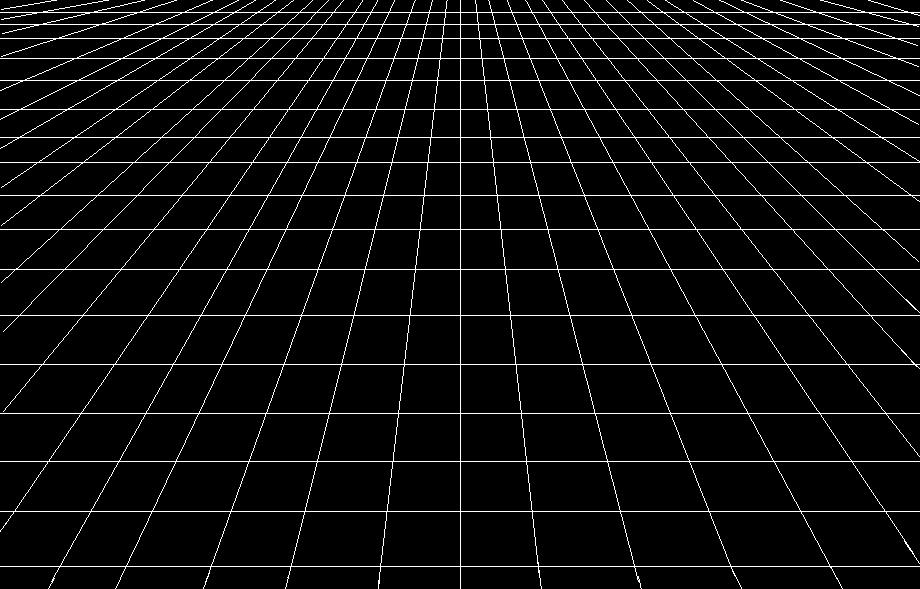
\includegraphics[width=0.5\textwidth]{flat-spacetime.jpeg}
\caption{\label{fig:flat}Flat Spacetime}
\end{figure}

\end{frame}

\begin{frame}
\frametitle{General Relativity: Some Basic Concepts}

\begin{itemize}
\item A generalization of Special Relativity (hence its name) which includes all sorts of spacetime distortions such as acceleration or gravitational fields
\item Massive objects create a ``dent'' or distortion in spacetime which is felt as gravity
\item Rotation of massive objects can also twist and distort spacetime
\end{itemize}

\begin{figure}
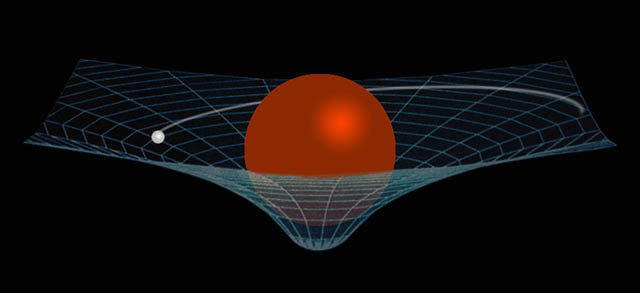
\includegraphics[width=0.5\textwidth]{Gravity.jpg}
\caption{\label{fig:gravity}A star causing a dent in spacetime - this is gravity}
\end{figure}

\end{frame}

\begin{frame}
\frametitle{Similarities between Special and General Relativity}

In case you haven't noticed, both of them deal with physics phenomena on a very large scale. These two theories seem to totally break down on the subatomic scale.

\bf{And this is where quantum mechanics comes in.}

\end{frame}

\section{Quantum Mechanics}

\begin{frame}
\frametitle{Quantum Mechanics}
\end{frame}

\begin{frame}
\frametitle{Background History}

\begin{itemize}
\item \emph{No definite date} for discovery of quantum mechanics
\item Phrase ``Quantum Mechanics'' coined by Max Born, Werner Heisenberg and Wolfgang Pauli in early 1920s
\item Other scientists who contributed to this theory include:
\begin{itemize}
\item Max Planck
\item Albert Einstein
\item Niels Bohr
\item Louis de Broglie
\item Paul Dirac
\item Erwin Schrodinger
\item Richard Feynman
\end{itemize}
\end{itemize}

\end{frame}

\begin{frame}
\frametitle{Some Basic Concepts}
\begin{itemize}
\item Theory for physical phenomena at the subatomic scale
\item Based purely on probability - there is no certainty anywhere in this theory
\item Major Concept: Wave-Particle Duality - Subatomic particles exhibit wave properties at times and particle properties at other times
\end{itemize}

\bf{As you zoom out of the subatomic scale, the probabilities average out so classical physics hold true on a large scale.}
\end{frame}

\begin{frame}
\frametitle{Double Slit Experiment}
\begin{itemize}
\item An experiment devised to demonstrate the wave-particle duality nature of subatomic particles
\item Also known as \bf{Young's Experiment}
\end{itemize}

First, a laser beam is shot at a plate containing 2 parallel slits. The light passing through the slits are observed on a screen behind the plate.

We find out that:

\begin{enumerate}
\item The light passing through the two slits interfere with each other - suggesting that light is a wave
\item However, when observed, each photon (light particle) passes through 1 slit only - suggesting that light is comprised of particles
\end{enumerate}

\end{frame}

\begin{frame}
\frametitle{Double Slit Experiment - Diagram}
\begin{figure}
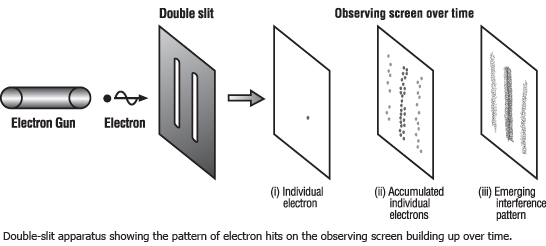
\includegraphics[width=\textwidth]{double-slit-experiment.jpg}
\caption{\label{fig:experiment}The Double Slit Experiment}
\end{figure}

\end{frame}

\begin{frame}
\frametitle{Problem}

These two theories have been proven time to time to be mutually incompatible, but both of them are completely valid!

\end{frame}

\section{String Theory and M-Theory}

\begin{frame}
\frametitle{String Theory and M-Theory}
\end{frame}

\begin{frame}
\frametitle{Background History}
\begin{itemize}
\item ``Prototype'' of String Theory discovered by Gabriele Veneziano during the 1950s/1960s
\item Originally used to explain hadron physics
\item Later adapted to explain all elementary particles - key theorists include Pierre Ramond, Andre Neveu, John Schwarz and Joel Scherk
\item There are currently \bf{5 different self-consistent string theories}
\end{itemize}
\end{frame}

\begin{frame}
\frametitle{Aims of String Theory}
\begin{enumerate}
\item Unite the 2 major theories of the universe, namely General Relativity and Quantum Mechanics
\item To create a single unified theory that explains \emph{everything}
\end{enumerate}
\end{frame}

\begin{frame}
\frametitle{Some Basic Concepts}
\begin{itemize}
\item All subatomic particles are composed of vibrating filaments of energy called strings
\item The difference between different subatomic particles and forces is due to the difference in the vibration of the string(s) - the strings themselves are pretty much the same
\item String Theory requires that there are \emph{10 dimensions} because in 3 dimensions, the number of ways that the strings vibrate (i.e. the dimensions in which they are vibrating, left-right, front-back, up-down and so on) are not enough for all of the particles and forces that exist in the universe
\item We cannot see the extra dimensions because they are curled up into very small spaces or we are living in a 3D subspace of a 10D manifold.
\end{itemize}
\end{frame}

\begin{frame}
\frametitle{M-Theory and ``Pea Brains''}

Since there are 5 string theories (hardly a unified theory, right?), M-theory is the theory that attempts to unify all 5 different string theories.

M-theory suggests that different-dimensional branes exist. For example, strings (1-branes) are one type of brane that exist, but there are also 2-branes, 3-branes and so on, up to 5-branes. The general term for all such branes are p-branes (read as ``pea brains'') where p is the dimension of the brane.

\begin{figure}
\centering
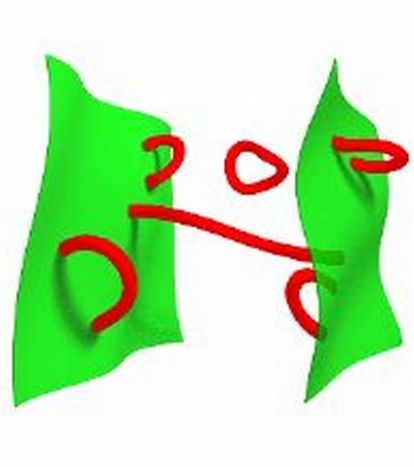
\includegraphics[width=0.25\textwidth]{p-branes.jpg}
\caption{\label{fig:branes}Membranes (2-branes) and Strings (1-branes) are just two of many types of p-branes}
\end{figure}

\end{frame}

\begin{frame}
\frametitle{Prerequisites of String/M-Theory}

An important prerequisite (i.e. assumption) of this theory is that there must be at least 6 other spatial dimensions that are unobservable on top of the 3 spatial dimensions and 1 time dimension that we can easily observe.

\end{frame}

\begin{frame}
\frametitle{Next ... }
Choose 1: \emph{Spinoff} or \emph{Credits}
\end{frame}

\section{Spinoff: Hyperdimensionality and God}

\begin{frame}
\frametitle{Spinoff: Hyperdimensionality and God}
\end{frame}

\begin{frame}
\frametitle{God - A Hyperdimensional Being?}

Before we continue, let us see what the Christian Bible says about the properties of God.

God is:

\begin{enumerate}
\item Omnipotent
\item Omniscient
\item Omnipresent
\end{enumerate}

Apart from that, the universe cannot contain Him.

\end{frame}

\begin{frame}
\frametitle{Demonstration of Omniscience}
\alert{LOOK AT THE WHITEBOARD AND PRESENTER!}
\end{frame}

\begin{frame}
\frametitle{Demonstration of Omnipresence}
\alert{LOOK AT THE WHITEBOARD AND PRESENTER!}
\end{frame}

\begin{frame}
\frametitle{``The universe cannot contain Him''}
\alert{LOOK AT THE WHITEBOARD AND PRESENTER!}
\end{frame}

\section{Credits}

\begin{frame}
\frametitle{Credits}
\end{frame}

\begin{frame}
\frametitle{Special and General Relativity}
\begin{itemize}
\item \url{https://en.wikipedia.org/wiki/General_relativity}
\item \url{http://www.space.com/17661-theory-general-relativity.html}
\item \url{https://en.wikipedia.org/wiki/Special_relativity}
\end{itemize}
\end{frame}

\begin{frame}
\frametitle{Quantum Mechanics}
\begin{itemize}
\item \url{https://en.wikipedia.org/wiki/Quantum_mechanics}
\item \url{https://en.wikipedia.org/wiki/History_of_quantum_mechanics}
\item \url{https://simple.wikipedia.org/wiki/Quantum_mechanics}
\item \url{https://en.wikipedia.org/wiki/Double-slit_experiment}
\end{itemize}
\end{frame}

\begin{frame}
\frametitle{String and M-Theory}
\begin{itemize}
\item \url{http://www.physlink.com/Education/AskExperts/ae138.cfm}
\item \url{http://www.columbia.edu/cu/record/23/18/14.html}
\item \url{http://www.dummies.com/how-to/content/the-basic-elements-of-string-theory.html}
\item \url{http://www.dummies.com/how-to/content/string-theory-for-dummies-cheat-sheet.html}
\item \url{https://en.wikipedia.org/wiki/Introduction_to_M-theory}
\item \url{https://en.wikipedia.org/wiki/String_theory}
\end{itemize}
\end{frame}

\begin{frame}
\frametitle{Thank You}

Thank you for listening!

\end{frame}

\begin{frame}
\frametitle{Alternate Versions}
\begin{itemize}
\item \url{http://donaldkellett.github.io/AS-Physics/introduction-ppt}
\item There is also a Google Slides version, but pasting the link here caused problems.  Go to the Slidex Version and the link to the Google Slides version should be there.
\end{itemize}
\end{frame}

\end{document}